\documentclass[12pt]{article}
\usepackage[utf8]{inputenc}
\usepackage[margin=1in]{geometry}
\usepackage{graphicx}
\usepackage{hyperref}
\usepackage{fancyhdr}
\usepackage{setspace}
\usepackage{amsmath}

\onehalfspacing

% Header and Footer
\setlength{\headheight}{14.49998pt}
\pagestyle{fancy}
\fancyhf{}
\rhead{\thepage}
\lhead{MCTS Project Report}

\title{\textbf{Budget AlphaGo on an old Laptop}}
\author{Alyx Liao \and Raphaël Giraud}
\date{\today}

\begin{document}

% Front Page
\begin{titlepage}
    \centering
    \vspace*{2cm}
    
    {\Large \textbf{Master IASD}}
    
    \vspace{1cm}
    
    {\large Lecture: MCTS}
    
    \vspace{3cm}
    
    {\Huge \textbf{Budget AlphaGo on an old Laptop}}
    
    \vspace{2cm}
    
    {\Large \textit{A miniature implementation of AlphaGo's MCTS algorithm, optimized for low computational resources.}}
    
    \vspace{3cm}
    
    {\large
        \begin{tabular}{c}
            Alyx Liao \\
            Raphaël Giraud
        \end{tabular}
    }
    
    \vspace{2cm}
    
    {\large April 2026}
    
    \vfill
\end{titlepage}

% Abstract
\newpage
\section*{Abstract}

This report presents the development of an AlphaGo-inspired neural network model trained with Monte Carlo Tree Search on a single laptop. The primary objective was to create the best performing Go-playing agent possible under strict hardware constraints: training on a single laptop equipped with an RTX 5080 GPU.
\newpage

% Table of Contents
\tableofcontents
\newpage

% Introduction
\section{Introduction}

\subsection{Motivation: The Bitter Lesson}

In his influential 2019 post ``The Bitter Lesson,'' Richard Sutton~\cite{sutton2019} reflects on decades of artificial intelligence research and concludes that the most reliable path to better AI systems lies not in incorporating domain knowledge or designing clever algorithms, but in maximizing the use of available computational resources combined with general-purpose learning methods. Sutton argues that AI researchers often spend considerable effort tuning hyperparameters and pursuing novel algorithmic ideas, only to find that simply scaling computation with existing methods yields superior results.

This project is motivated directly by this observation. Rather than pursuing exotic new techniques or exhaustively tuning every hyperparameter, we focus on efficiently leveraging the computational power available on a single laptop to train the strongest Go-playing agent possible. We believe that thoughtful, disciplined use of available hardware resources—applying modern training techniques systematically and scaling search appropriately—can produce compelling results without requiring access to large-scale distributed systems.

\subsection{Background}

\subsubsection{Monte Carlo Tree Search and Neural Networks}

Monte Carlo Tree Search (MCTS) is a decision-making algorithm that has become fundamental in game-playing artificial intelligence. MCTS combines tree search with random sampling, expanding the search tree toward the most promising moves through iterative evaluation. The algorithm gained widespread prominence following the release of AlphaGo~\cite{silver2016}, which achieved a major milestone by defeating professional Go players through the combination of MCTS with deep neural networks.

Subsequent work introduced AlphaGo Zero~\cite{silverzero2017}, which removed the need for human game data entirely, instead learning through pure self-play with MCTS. AlphaZero~\cite{silveralphazero2018} generalized this approach to other games (chess, shogi), cementing the effectiveness of neural-network-guided MCTS as a state-of-the-art paradigm.

\subsubsection{The Implementation Gap}

Despite the remarkable empirical results and widespread citations of these landmark papers, a critical gap exists: neither the original AlphaGo, AlphaGo Zero, nor AlphaZero papers provide publicly available source code or detailed implementation specifications. While the papers present the high-level algorithmic framework, they conspicuously omit crucial implementation details essential for reproducibility:

\begin{itemize}
    \item \textbf{Batch inference architecture}: How are neural network evaluations batched during tree search? What inference server architecture enables efficient GPU utilization during parallel tree expansion?
    \item \textbf{Programming language and framework choices}: Which languages implement the tree search, replay buffer, and training loop? What concurrency primitives are used?
    \item \textbf{Parallelism strategies}: Are tree-level, root-level, or leaf-level parallelization schemes employed? How is thread safety managed?
    \item \textbf{Memory management}: How are replay buffers sized and managed? What strategies minimize memory overhead during self-play?
    \item \textbf{Training infrastructure}: What is the exact orchestration between data generation (self-play), model updates, and inference serving?
\end{itemize}

\subsubsection{Open-Source Implementations and Prior Work}

To address this gap, the machine learning community has produced numerous open-source AlphaZero-inspired implementations: alpha-zero-general (suragnair), AlphaZero\_Gomoku (junxiaosong), LightZero (OpenDiLab, NeurIPS 2023 Spotlight), and CrazyAra (chess engine in C++/Python). These implementations provide valuable reference code, though they vary significantly in architectural choices, programming languages, and parallelization strategies.

Work on parallel MCTS has been studied since at least 2008~\cite{chaslot2008}, with three main parallelization paradigms identified: leaf parallelization (parallel playouts from one tree node), root parallelization (independent trees merged at root), and tree parallelization (shared tree with synchronization). Lock-free approaches have also been explored~\cite{enzenberger2010}. However, most literature focuses on the algorithmic aspects rather than practical system-level implementations.

\subsubsection{Project Positioning}

This project directly addresses the implementation gap. Rather than relying on abstract high-level descriptions, we document explicit architectural choices: dual-language design (Python for training/inference serving, Go for interactive gameplay), gRPC for client-server communication, specific parallelism handling, and pragmatic memory management on a single laptop. By prioritizing careful resource utilization rather than novel algorithms, we provide a concrete reference implementation that others working under similar hardware constraints can learn from or adapt.

\subsection{Objectives}

Motivated by the Bitter Lesson and a deep personal connection to Go, our objectives are:

\begin{itemize}
    \item \textbf{Train an agent that plays sensibly}: Develop a neural network with learned value and prior probabilities good enough that, when combined with MCTS at modest simulation budgets (200--3200 sims/move), produces moves that appear thoughtful rather than random to the human eye. The agent should be capable of calculating several moves ahead through guided search, demonstrating genuine game understanding rather than mere pattern matching.
    
    \item \textbf{Have fun and close a personal circle}: One of the authors, Alyx, grew up playing Go with her father—a game deeply woven into her childhood. In March 2016, DeepMind's AlphaGo defeated world champion Lee Sedol, a watershed moment that profoundly affected her as both a Go player and someone who had just begun learning to code. This project is an homage to that inspiration: attempting, on a modest single laptop, to create our own budget AlphaGo and meaningfully engage with the algorithms that sparked a fascination with AI and computer science.
\end{itemize}

\section{Environment Simulation: Implementing Go}

Our system implements a correct Go game engine in the Go programming language (golang), which we learned from scratch for this project. While languages like C or C++ would offer superior raw performance, we chose Go for its elegant concurrency primitives, rapid development cycle, and for the charming coincidence that coding the game of Go in the Go language would be more enjoyable—and it was.

\subsection{Board State, Groups, and Move Legality}

The core of our game engine rests on a union-find (disjoint set) data structure that efficiently manages connected groups of stones. Each stone placed on the board begins as a singleton group with an associated liberty count. When a stone is placed adjacent to friendly stones (orthogonally neighboring), groups are merged using union by rank to maintain logarithmic-time operations through path compression. This elegant structure lets us track group membership in near-constant amortized time, maintain accurate liberty counts as stones are captured or merged, and efficiently identify which groups are captured when a new stone is placed.

Move legality is enforced through three conditions: (1) the target cell must be empty, (2) the move must not be suicidal (the placed stone's group must have at least one liberty after placement, or the move must capture enemy stones), and (3) the move must not violate the superko rule, which we enforce via Zobrist hashing (see below). Legal moves are computed by iterating all board positions; resign and pass actions are always legal regardless of board state.

\subsection{Zobrist Hashing and Superko Rule}

To prevent infinite repetition through board state recurrence, we employ Zobrist hashing. Each cell-player combination is assigned a unique random 64-bit hash value. As the game progresses, the cumulative board hash is updated incrementally via XOR operations:

\begin{equation}
H_{\text{new}} = H_{\text{old}} \oplus ZT[i][j][\text{stone}] \oplus P
\end{equation}

where $ZT[i][j][\text{stone}]$ is the Zobrist table entry for position $(i,j)$ and stone color, and $P$ is the player turn hash. A complete history of board hashes is maintained throughout the game, allowing us to reject any move whose resulting board state produces a hash that has appeared earlier. This simple yet powerful technique enforces the superko rule with negligible computational overhead.

\subsection{Game Termination and Scoring}

The game ends when either both players consecutively pass (indicating no more beneficial moves) or when a player resigns. Scoring follows Trump-Taylor (area) rules, consistent with AlphaGo~\cite{silver2016}: we count all stones on the board for each player, identify connected regions of empty cells via BFS, determine whether each empty region is surrounded exclusively by one color or both, and assign territory accordingly. Neutral regions (surrounded by both colors) count toward neither player. White's final score includes komi adjustment (6.5 points in our implementation). The winner is determined by comparing final scores; explicit resignation immediately determines the winner as the opponent of the resigning player.

\section{Parallel MCTS}

\subsection{Monte-Carlo Tree Search with Predictor Upper Confidence Tree}

Our agent combines MCTS with a value-prediction neural network via the PuCT (Predictor Upper Confidence Tree) algorithm, an approach closely related to AlphaGo's architecture. The algorithm maintains a search tree where each node represents a board state and edges represent actions. During each simulation, the tree is traversed from root to a leaf using the UCB formula:

\begin{equation}
UCB(s, a) = Q(s, a) + C \cdot P(s, a) \cdot \frac{\sqrt{N(s)}}{1 + N(s, a)}
\end{equation}

where $Q(s, a)$ is the mean value of the action, $N(s)$ and $N(s, a)$ are visit counts, $P(s, a)$ is the prior probability from the neural network, and $C$ is the exploration constant. Upon reaching a leaf or terminal node, the neural network evaluates the position and returns a value estimate. This value is then backpropagated through the tree, updating all traversed edges with the predicted outcome. Actions are selected deterministically via argmax in evaluation mode and via temperature sampling (biased toward higher visit counts) during training.

\subsection{Parallelization and Queue-Based Asynchronous Evaluation}

To accelerate simulation throughput despite GPU bottlenecks, we implemented multi-threaded tree search with lock-protected action selection. Each thread executes the MCTS loop independently, but all tree modifications are serialized through mutual exclusion locks around the \texttt{SelectChild} operation, ensuring consistent visit count updates and tree integrity.

Critically, we did not implement virtual loss, a technique commonly used to diversify exploration across threads. Instead, we relied on the natural penalization that occurs when incrementing visit counts: selecting an action increases its $N(s, a)$ denominator, reducing its UCB score on subsequent selection. This simple mechanism proved sufficient to prevent threads from repeatedly selecting identical actions, keeping the search diverse without explicit virtual loss overhead.

To decouple neural network latency from tree search, we employed a queue-based architecture: when a thread reaches a leaf node, it enqueues the position for evaluation and immediately resumes tree search using upper tree estimates. A background gRPC client processes the queue asynchronously, receiving evaluations from the Python server and writing results back into the tree. This asynchronous design allowed threads to continue working even while the network was busy, dramatically improving CPU utilization and throughput.

\subsection{Throughput and Scaling Characteristics}

Without neural network overhead, UCT with rollout-based evaluation requires expensive random playouts to terminal states. Even with these expensive rollouts, we achieved approximately 2000 simulations per second using parallel search with lock-protected selection—suggesting that without rollouts, throughput would exceed 9000 simulations per second. However, once neural network evaluation was introduced, GPU operations became increasingly expensive (despite being faster than random rollouts), reducing the practical simulation rate to approximately 1200 simulations per second. Paradoxically, enabling parallelism with PuCT did not improve throughput; the optimal configuration was 1 parallel search thread, which avoided lock contention and queue congestion.

\subsection{Parallelization Issues and Terminal Node Overestimation}

During development, we discovered a critical bug in the interaction between parallelism and neural network inference. When positions reached terminal game states (e.g., both players passing), evaluating these positions is instant (game already scored), whereas non-terminal positions must await network evaluation from the server. This asymmetry caused a pathological behavior: one thread would rapidly select and re-explore a terminal node while other threads were blocked waiting for network responses to their non-terminal evaluations. The terminal node's visit count would become severely inflated, and its value would be dramatically misestimated as its high visitation made it appear attractive in the UCB formula, despite being a losing terminal state.

The fix was simple but non-obvious: submit terminal nodes to the neural network for evaluation anyway, even though the true game outcome is already known. When the evaluation returned, we immediately overwrote it with the actual game result. This ensured that all position types incurred similar evaluation latency, eliminating the incentive for threads to repeatedly explore terminal nodes. This is an example of how low-level implementation details in parallelization can silently introduce subtle biases into learning algorithms—a lesson that rarely appears in published research.

\section{Training Pipeline}

\subsection{Model Architecture}

The neural network is a residual convolutional architecture (Gogo81) with approximately 1.5M parameters. It processes 4-plane board history (current and past 3 moves) through an input projection to 96 channels, 15 residual blocks with layer normalization, and two output heads. The policy head predicts move probabilities over 83 actions (81 board + pass + resign); the value head predicts outcome in $[-1, 1]$ via tanh. Both heads incorporate metadata (player color and enemy pass count). The architecture prioritizes efficient inference and feature reuse across both objectives.

\subsection{gRPC-Based Client-Server Communication}

The system uses a dual-process architecture: Go client (game engine + MCTS) and Python server (training + inference) communicate via gRPC~\cite{google_grpc} with Protocol Buffers~\cite{google_protobuf} serialization. The connection uses a \textbf{Linux Unix Domain Socket} at {\ttfamily /tmp/\allowbreak position\_evaluator.\allowbreak sock}, offering lower latency than TCP for localhost. This platform-specific choice (Windows incompatible) was acceptable for development but would require TCP refactoring for cross-platform deployment.

Importantly, while the final configuration uses only 1 MCTS thread for optimal throughput, the parallel infrastructure was essential to achieve batching efficiency. With multiple threads submitting evaluation requests concurrently, the server's batching queue filled naturally, enabling the 50 ms timeout-based adaptive batching scheme described below. Serial single-threaded evaluation would require either artificial request accumulation or large timeouts, both of which would hurt latency. Thus, multithreading was instrumental to the batching design, even though the search itself runs single-threaded.

\subsection{Experience Replay and Data Augmentation}

After each completed self-play game, the Go client submits all positions encountered (state, action probabilities from MCTS visit counts, game outcome value) to the Python training server. These are stored in a replay buffer of capacity 800,000 experiences, optimized through aggressive quantization: boards and masks are stored as int8/uint8, policy distributions as float16. When the buffer reaches a threshold of 32,768 new experiences, training begins.

Crucially, each submitted experience is augmented with all 8 symmetries: 4 rotations and horizontal flips thereof. This data augmentation expands each game's 40--60 positions into 320--480 training examples, improving sample efficiency and enabling the 12:1 replay ratio (training on 12 samples per collected experience).

\subsection{Training Phases}

Training follows two phases following each game submission:

\begin{enumerate}
    \item \textbf{Experience Accumulation}: Positions are collected from self-play and buffered until reaching 32,768 new post-game experiences. A progress bar tracks accumulation.
    \item \textbf{Post-Game Training}: After a game completes and reaches the threshold, a training phase runs consuming $12 \times N_{\text{new}}$ samples (where $N_{\text{new}}$ is the number of new experiences). Batches of 512 are drawn via uniform sampling from the replay buffer. Each batch is passed through the model (forward pass), and losses are computed:
    \begin{align}
        \mathcal{L}_{\text{total}} &= \alpha \cdot \mathcal{L}_{\text{value}} + \mathcal{L}_{\text{policy}} \\
        \mathcal{L}_{\text{value}} &= \text{MSE}(v_{\text{pred}}, v_{\text{target}}) \\
        \mathcal{L}_{\text{policy}} &= -\sum_{a} p_{\text{target}}(a) \log \pi_{\text{pred}}(a)
    \end{align}

    where $\alpha = 1.0$ (equal weighting). The optimizer is Adam with base learning rate $3 \times 10^{-4}$, weight decay $10^{-4}$, using warmup ($100$ steps linear, then cosine annealing) and bfloat16 mixed precision on GPU.
\end{enumerate}

\subsection{Inference Batching with Timeouts}

The inference server must handle evaluation requests arriving sporadically from multiple MCTS threads. Naive inference (one forward pass per request) would be inefficient; batching is essential for GPU utilization. However, if we wait indefinitely for full batches, MCTS threads will block on network latency.

Our solution uses timeout-based adaptive batching: requests accumulate in a queue; a batch is executed when either (i) the queue reaches 20 requests (batch size), or (ii) the batch timeout expires. The batch timeout is set to 50 ms—conservative enough that batches usually fill before timeout, yet short enough that unblocked threads resume quickly. A background monitoring thread periodically checks batch age and flushes partial batches, ensuring requests don't stall indefinitely even under low traffic.

This design worked remarkably well in practice. Timeouts proved more pragmatic than alternative schemes (e.g., deterministic batch sizes, full-queue-only flushing) which led to either CPU underutilization or MCTS stalling. We found 50 ms to be an optimal balance discovered through empirical iteration.

\section{Results}

\subsection{Training Configuration and Progression}

Self-play training employed the following hyperparameters: each move during self-play was selected via MCTS with 400 simulations per move and temperature-based sampling (exploration during training). Players could resign if the best move's value fell below $-0.9$ (estimate of $\sim 80\%$ win probability deficit), enabling faster game termination and reducing computational waste on lost positions.

The replay buffer capacity was set to 800,000 positions, maintained in a FIFO (first-in-first-out) manner with continuous recycling. Over the full training duration, 3,600,000 self-play positions were collected and cycled through the buffer—4.5 times the buffer capacity—ensuring diverse experience coverage without requiring prohibitively large memory. This rolling buffer approach risks catastrophic forgetting, where the model unlearns earlier-learned patterns. However, empirically, the training curves (Figure~\ref{fig:training}) show no signs of loss spikes or divergence that would indicate catastrophic forgetting. The monotonic loss decrease suggests that the fundamental task (predicting game outcomes and action probabilities) remains learnable across the evolving dataset, and that the experience diversity from continuous buffer cycling sufficed to prevent overfitting to a stale dataset.

Training data was collected during self-play at an average rate of 28 positions per second, yielding approximately $3,600,000 / 28 \approx 128,571$ seconds of collection, or roughly 35.7 hours of self-play games. The subsequent optimization phases (training on the accumulated replay buffer with 12:1 replay ratio) consumed an additional 2.9 hours, for a total wall-clock time of approximately 38.6 hours of training.

Training proceeded over 111 phases, accumulating 85,994 optimization steps. Figure~\ref{fig:training} visualizes the loss trajectories and learning rate schedule. The total loss decreased monotonically from $\sim 3.2$ to $\sim 2.7$, with the minimum achieved at step 79,335. Value loss (MSE on game outcomes) remained relatively stable around $0.15$--$0.17$, while policy loss (cross-entropy on MCTS visit distributions) converged from $3.1$ to $\sim 2.6$, indicating that the model learned to better emulate the MCTS distributions over time.

The learning rate schedule followed a linear warmup for 100 steps, then cosine annealing over 100,000 steps total, with a minimum learning rate floor of $3 \times 10^{-6}$. This conservative schedule prevented aggressive parameter updates that could disrupt learned representations.

\begin{figure}[h]
\centering
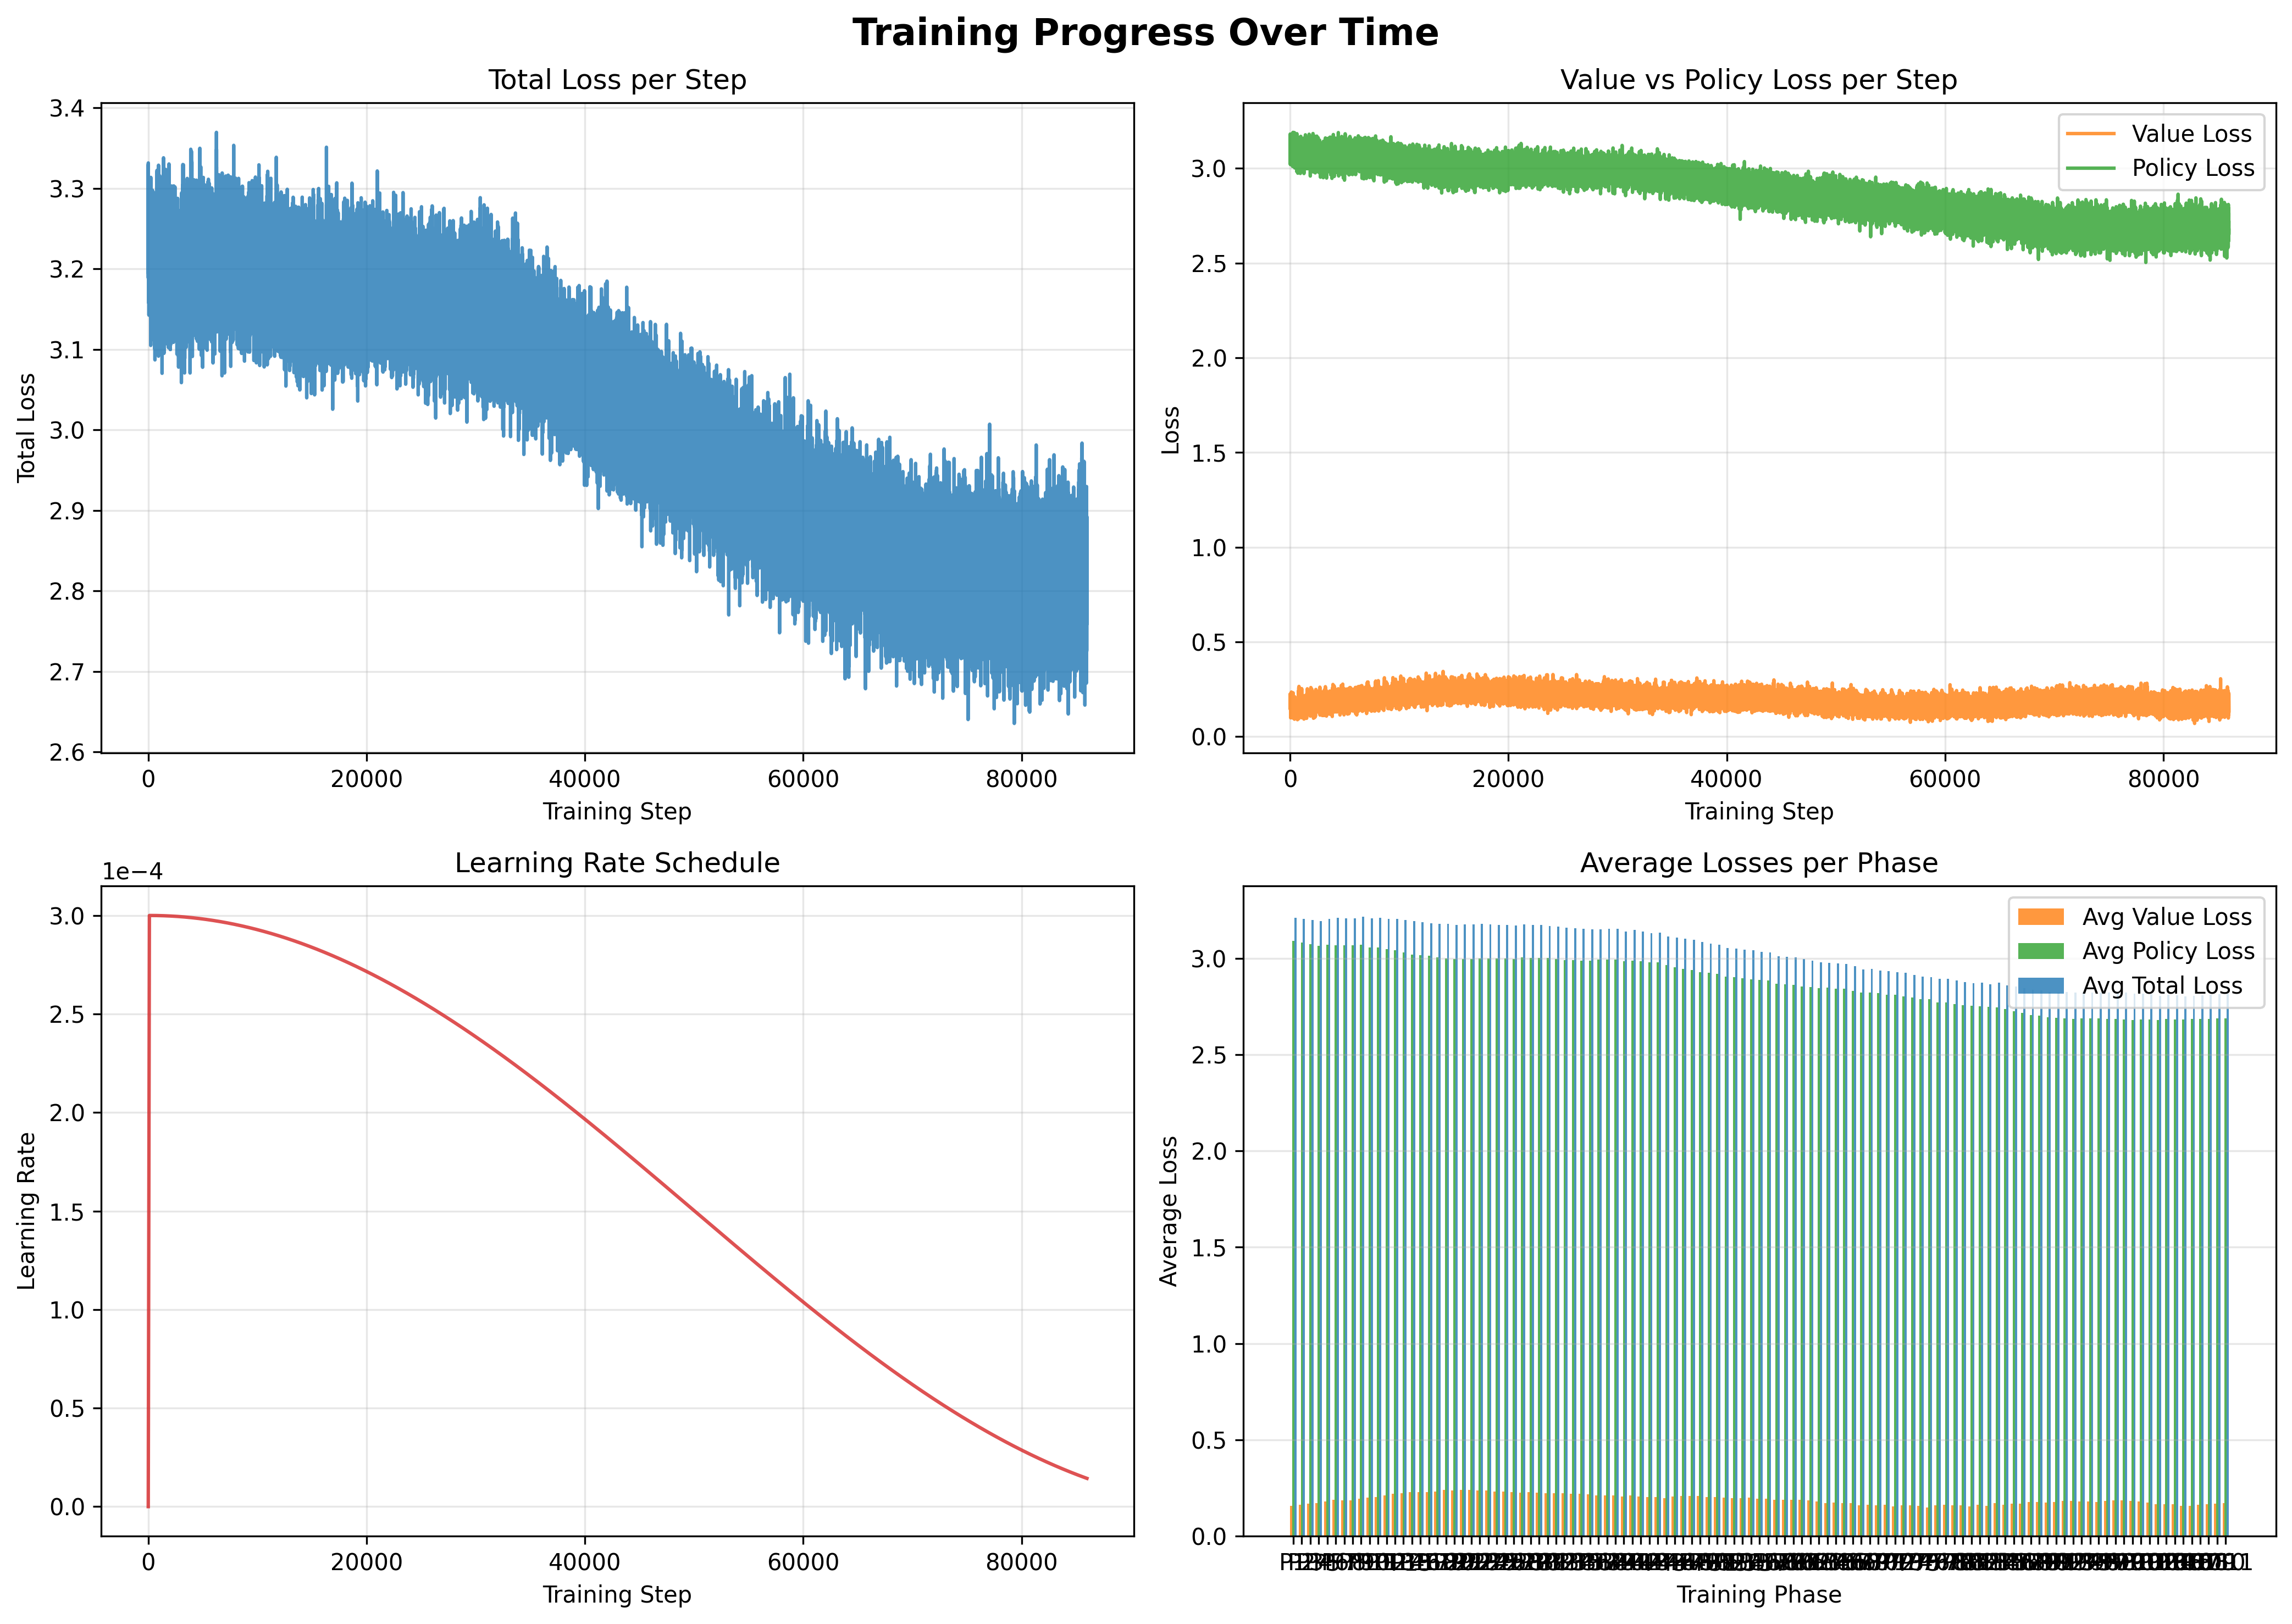
\includegraphics[width=0.95\textwidth]{training_logs.png}
\caption{Training loss and learning rate progression. \textit{Top left:} Total loss per step showing convergence trend. \textit{Top right:} Value vs policy loss decomposition. \textit{Bottom left:} Learning rate schedule with linear warmup and cosine decay. \textit{Bottom right:} Phase-wise averages showing stability across training phases.}
\label{fig:training}
\end{figure}

\subsection{Tournament Comparisons}

We conducted a round-robin tournament comparing MCTS agents at three computational budgets: 200, 800, and 3200 simulations per move. Each agent pair played 10 games in self-play (diagonal entries) and 20 games in cross-play (10 as black, 10 as white). The results are presented in Table~\ref{tab:tournament}.

\begin{table}[h]
\centering
\caption{Tournament Results: Winrate Table (Rows vs Columns). Each cell shows ``Row Agent as Black \% / Row Agent as White \%''. Self-play entries (diagonal) indicate the agent's winrate when playing itself.}
\label{tab:tournament}
\begin{tabular}{c|ccc}
\hline
\textbf{Sims} & \textbf{200} & \textbf{800} & \textbf{3200} \\
\hline
\textbf{200}  & 80.0\% / 20.0\% & 100.0\% / 0.0\% & 90.0\% / 0.0\% \\
\textbf{800}  & 100.0\% / 0.0\% & 100.0\% / 0.0\% & 100.0\% / 0.0\% \\
\textbf{3200} & 90.0\% / 10.0\% & 100.0\% / 0.0\% & 90.0\% / 10.0\% \\
\hline
\end{tabular}
\end{table}

The results reveal a critical flaw in the trained model: the network exhibits severe color asymmetry. White winrates are dramatically lower than Black winrates across all strength levels, and critically, the model is essentially unable to win as White (0\% or near-0\% in most cross-play scenarios). This represents a fundamental training failure rather than a skill difference between colors—the model should learn that competent moves exist for both colors.

We attribute this to a shortcoming in the model architecture: player color ($\pm 1$) is specified as a single scalar input feature concatenated to the policy and value head outputs, rather than being embedded early in the network and incorporated throughout. This minimal color encoding likely fails to propagate color information through the residual trunk, causing the convolutional features to conflate Black and White patterns. The model appears to have collapsed toward a Black-centric policy early in training and lacked sufficient architectural channels to correct this bias. However, we acknowledge uncertainty in the root cause. An alternative explanation is that Go's inherent property—where winning as White becomes significantly more difficult if the komi (compensation) is too low—contributed to the bias. If the chosen komi of 6.5 was insufficient relative to Black's first-move advantage at certain stages of training, the model may have encountered a prolonged period where White positions were genuinely disadvantageous, biasing the learned policy toward Black. 

A third hypothesis involves a self-reinforcing negative feedback loop: as the network's value estimates labeled White positions as progressively worse (following suboptimal play), the policy head learned pessimism about White's prospects. This learned pessimism then caused the MCTS selection mechanism to explore White moves with lower priority, resulting in genuinely weaker White play in subsequent self-play games. These weaker outcomes would then reinforce the value estimates' pessimism about White, creating a cycle where the network's own predictions became self-fulfilling. Such feedback loops are difficult to escape during training because the value estimates—which drive both MCTS selection and policy learning—become corrupted by their own circular reasoning.

Distinguishing among these hypotheses (architectural inadequacy, insufficient komi, or self-reinforcing feedback) would require controlled experiments with varied architectural designs, komi values, and potentially techniques to break the feedback loop (e.g., alternating komi values across games or adding regularization to prevent extreme value estimates).

\section{Conclusion}

The final trained agent, despite the Black/White asymmetry, demonstrates reasonable play from a human perspective. While not superhuman—and indeed far from competitive with professional or even intermediate human players—the agent's ability to select coherent moves after exploring hundreds of simulated futures represents a qualitative leap beyond random play. Observing a neural network trained on a budget laptop make sensible positional and tactical decisions is genuinely impressive.

This project represents the culmination of significant learning and engineering effort. We mastered Go's rules and scoring, implemented Protocol Buffers and gRPC communication, and—most ambitiously—implemented a functional MCTS with PuCT value guidance entirely from first principles, using only the AlphaGo and AlphaZero papers as reference. Implementing MCTS with neural network integration is non-trivial; the correct handling of parallelism, asynchronous queue-based evaluation batching, and the subtle bugs we discovered (terminal node overestimation, color bias in value estimates) underscore the complexity of systems-level machine learning implementation that papers often elide.

We are immensely proud of this project. Within the constraints of a single laptop, we implemented a complete AlphaGo-inspired training pipeline from data generation through self-play to model refinement, focusing on careful implementation and thoughtful resource utilization. The Black/White asymmetry remains an open question, but the investigation itself—considering architectural, game-theoretic, and feedback-loop explanations—demonstrates the kind of analytical thinking required to debug deep learning systems in the wild. For students learning MCTS, neural network training, or Go, we hope this project serves as a concrete, reproducible reference implementation.

% Bibliography
\bibliographystyle{ieeetr}
\bibliography{references}

\end{document}